\documentclass[a4paper,review,12pt,authoryear]{elsarticle}

% \usepackage{natbib}
\usepackage{amsfonts,amsmath,bbm,bm,xcolor,booktabs,hyperref,amsthm}
\usepackage{geometry}
\usepackage{subfig}
\geometry{a4paper,scale=0.8}
\usepackage{setspace}
\setstretch{1.5}
\let\code=\texttt
\let\proglang=\textsf
\setcounter{MaxMatrixCols}{20}

\hypersetup{
  colorlinks=true,
  linkcolor=blue,
  citecolor=blue,
  urlcolor=blue}

% ADDING LINENUMBERS FOR REVIEWING:
% \usepackage{lineno}

\begin{document}

\begin{frontmatter}

  \title{On the performance of hierarchy construction: impacts of structure and clustering}

  \author[label1]{Bohan Zhang\corref{cor1}}
  \address[label1]{School of Economics and Management, Beihang University, Beijing, China}
  \ead{zhangbohan@buaa.edu.cn}
  \cortext[cor1]{Corresponding author.}
  \author[label2]{Anastasios Panagiotelis}
  \address[label2]{The University of Sydney Business School, NSW 2006, Australia}
  \author[label3]{Han Li}
  \address[label3]{Centre for Actuarial Studies, Department of Economics, The University of Melbourne, Australia}

  \begin{abstract}

    Forecast reconciliation has attracted significant research interest in recent years, with most studies relying on pre-defined hierarchies based on time series metadata. With the goal of forecast performance in mind, we extend the existing literature on clustering-based reconciliation approach by proposing a novel framework based on hierarchy construction approaches. This framework offers three variants: cluster hierarchies, random hierarchies, and combination hierarchies. Utilizing the proposed approaches, we investigate the individual contributions of two primary factors, namely clustering and enriched structure, to the performance of forecast reconciliation.  Through a simulation study and experiments on two real-world datasets, we demonstrate the practical efficacy of hierarchy construction approaches. Our findings provide new insights into the dynamics between clustering and enriched structure, significantly enriching our understanding of forecast reconciliation.


  \end{abstract}

  \begin{keyword}
  Forecasting \sep
  Hierarchical time series \sep
  Clustering \sep
  Hierarchy construction \sep
  Forecast combination
  \end{keyword}

\end{frontmatter}

%\clearpage
\newpage
% \linenumbers

\section{Introduction}

Hierarchical time series (HTS) has various important applications ranging from supply chain management (\citealp{syntetosSupplyChainForecasting2016}) to tourism (\citealp{kourentzesCrosstemporalCoherentForecasts2019}), electrical load (\citealp{jeonProbabilisticForecastReconciliation2019}), retail demand (\citealp{makridakisM5AccuracyCompetition2022}) forecasting. In recent decades, there has been an increasing interest in hierarchical forecasting, primarily driven by the success of the optimal reconciliation framework (\citealp{hyndmanOptimalCombinationForecasts2011,wickramasuriyaOptimalForecastReconciliation2019, panagiotelisProbabilisticForecastReconciliation2023}). Unlike the traditional approaches such as bottom-up and top-down, which generate coherent forecasts using forecasts from a single level, the reconciliation framework optimally combine base forecasts of all series in HTS. Numerous case studies in the literature demonstrate that reconciliation approaches not only yield coherent forecasts but also enhance overall forecast performance (\citealp{AthanasopoulosForecastReconciliationReview2023}).

The primary objective of hierarchical forecasting is to produce coherent forecasts for the series within a given HTS, which we refer to as \textit{original hierarchy}, ensuring that decision-makers at different levels of the hierarchy can analyze and make informed decisions based on aligned expectations for the future.
Consequently, the majority of existing research in forecast reconciliation literature experiments on the original hierarchy, which is typically formed according to inherent attributes of the bottom-level series, such as geographical location, gender, product category, travel purpose, and others. This limitation is evident in the absence of any discussion regarding cluster-based approaches in the recent comprehensive review of forecast reconciliation by \cite{AthanasopoulosForecastReconciliationReview2023}. However, the question arises as to whether the original hierarchy is the optimal structure and whether better structure can be constructed when pursuing superior forecast performance.  This inquiry serves as the key motivation behind the investigation presented in this paper.

Two observations have been consistently demonstrated in empirical studies on forecast reconciliation. First, the accuracy of base forecasts, which are influenced by the individual time series characteristics within the hierarchy, critically affects the overall performance of reconciliation.  Second, performance improvements achieved through reconciliation do not occur across all levels of the hierarchy. In fact, gains for some series often come at the expense of others.
These observations have motivated researchers to explore the idea of enriching the original hierarchy by introducing new time series via clustering analysis.
The rationale behind this approach lies in grouping time series with similar patterns together, thereby creating parent time series with stronger signals and consequently, improved forecastability. Ideally, the original series can ``borrow strength'' from the newly created series, leading to improved performance across all levels. For example, \cite{pangHierarchicalElectricityTime2022} propose a multiple alternative clustering method to group similar electricity and solar power time series.  In a similar vein, \cite{matteraImprovingOutofSampleForecasts2023} utilize Partition Around Medoids algorithms to unveil underlying structures in stock price indexes, while \cite{liForecastReconciliationApproach2019} apply agglomerative clustering to cause-of-death time series. These studies construct new hierarchies through clustering algorithms and demonstrate superior forecast performance compared to reconciliation without clustering, aligning with similar ideas from other research (e.g., \citealp{huberClusterbasedHierarchicalDemand2017, pangHierarchicalElectricityTime2018}). 
However, they are limited in scope as they concentrate solely on a specific time series clustering technique. To comprehensively investigate the effectiveness of clustering-based hierarchies, our approach involves a systematic comparison of multiple time series clustering techniques. This comparison incorporates a diverse set of time series representations, distance measures and clustering algorithms to provide a more thorough understanding of their impact on forecast performance.

Despite the intuitive appeal of clustering algorithms in forming parent time series with improved forecastability, uncertainties persist. Even if time series with superior forecastability are constructed, such improvements do not guarantee enhanced reconciliation performance, given the inherent uncertainty in estimating covariance matrices of base forecast errors (\citealp{pritulargaStochasticCoherencyForecast2021}). Therefore, the conclusion that clustering technique is the primary contributor to forecast performance improvement is not straightforward. 
The observed improvement could also be attributed to the enriched structure itself, where a larger set of series is optimally combined to obtain the reconciled forecasts, leading to reduced model uncertainty and data uncertainty.
To address these concerns, we propose a random hierarchy construction approach. By randomly constructing ``twin'' hierarchies with the same tree structure but different permutations of bottom-level series as a contrast to a clustering-based hierarchy, we are able to isolate the influence of clustering algorithms. This allows us to inspect the individual contributions of the enriched structure and clustering technique to forecast reconciliation performance.

Randomness technique is commonly integrated with forecast combination approaches in the forecasting literature. An illustrative instance is found in the work of \cite{bergmeirBaggingExponentialSmoothing2016}, who leverage a bootstrap aggregation (bagging) technique to improve the performance of exponential smoothing models. This involves combining forecasts derived from bootstrapped versions of the time series, demonstrating consistent superior performance on the M3 dataset. Additionally, \cite{petropoulosExploringSourcesUncertainty2018a} explore three sources of uncertainty, model uncertainty (data uncertainty and parameter uncertainty), and conclude that the efficacy of bagging technique stems from model uncertainty. To address the uncertainty introduced by random hierarchies, we propose a method that combines reconciled forecasts derived from multiple random hierarchies, assigning equal weights to each. Furthermore, for a fair comparison with clustering algorithms, we include an equally weighted combination of reconciled forecasts obtained from multiple cluster-based hierarchies.

This paper presents four main contributions:

\begin{itemize}
  \item We introduce a novel hierarchical forecast reconciliation framework centered on hierarchy construction.  Within this framework, we explore and compare three distinct approaches: cluster hierarchies, random hierarchies, and combination hierarchies.
  \item In contrast to existing literature that often focuses on a single clustering technique, our study systematically investigates the effectiveness of various time series clustering implementations. This investigation involves the incorporation of four time series representations, two distance measures, and two clustering algorithms.
  \item Through a simulation study featuring an artificial example, we illustrate a scenario wherein the enriched structure, rather than clustering, emerges as the primary contributor to forecast reconciliation performance. Another scenario highlights the importance of carefully selecting a clustering technique.
  \item We conduct experiments using two real-life datasets - the Australian tourism dataset and the U.S. cause-of-death mortality dataset. The results demonstrate the superior performance of hierarchy construction approaches, especially the combination hierarchies. Our research provides valuable insights into why clustering-based approaches enhance forecast reconciliation performance and offers guidance on the selection of hierarchy construction methods.
\end{itemize}

The rest of the paper is organized as follows. In section~\ref{sec:method} we introduce the proposed framework, elaborating on three approaches: cluster hierarchies, random hierarchies and combination hierarchies. The simulation study is presented in Section~\ref{sec:simulation}, while Section~\ref{sec:emp} details empirical experiments conducted on the Australian tourism dataset and U.S. mortality dataset. Finally, Section~\ref{sec:conclusion} concludes this paper with discussions on the findings and outlines future research directions.

\section{Methodology}
\label{sec:method}


In this section, we illustrate the proposed framework for hierarchy construction. We begin by introducing the necessary notations, followed by detailed explanation of the overall framework. The three subsections followed present cluster hierarchies (Section~\ref{sec:cluster}), random hierarchies (Section~\ref{sec:random}) and combination hierarchies (Section~\ref{sec:combination}), respectively. Section~\ref{sec:reconciliation} describes the procedure for reconciliation and evaluation. 

Given the original hierarchy, let $m$ and $n$ denote the number of time series in the bottom level and the hierarchy, respectively. Vectors $\boldsymbol{b}_t$ and $\boldsymbol{y}_t$ represent observations of bottom level and hierarchy at time $t$. They are linked through an $n\times m$ summing matrix $\boldsymbol{S}$, which can be decomposed into an identity matrix $\boldsymbol{I}_m$ and a constraint matrix $\boldsymbol{A}$, i.e., 
\[
  \boldsymbol{y}_t = \boldsymbol{S}\boldsymbol{b}_t = \begin{bmatrix}
    \boldsymbol{A} \\ \boldsymbol{I}_m 
  \end{bmatrix}  \boldsymbol{b}_t,
\]
where $\boldsymbol{A}$ represents the mapping from bottom-level time series to upper-level time series. While HTS can accommodate general linear constraints, this paper focuses specifically on the most common aggregation constraints, where the matrix $\boldsymbol{A}$ consists solely of $0$ and $1$.
We define hierarchy construction as the process of creating ``new middle-level series'', resulting in a modified HTS $\boldsymbol{y}^c_t$, which can be represented as:
\[
    \boldsymbol{y}^c_t = \boldsymbol{S}^c\boldsymbol{b}_t = \begin{bmatrix}
        \boldsymbol{A} \\
        \boldsymbol{C}_1' \\
        \vdots \\
        \boldsymbol{C}_K' \\
        \boldsymbol{I}_m
    \end{bmatrix}\boldsymbol{b}_t,
\] 
where each $\boldsymbol{C}_k$ represents a newly created middle-level series, formed by aggregating a subset of bottom-level series $\boldsymbol{b}_t$. The vector $\boldsymbol{C}_k$ is of $m$-dimensional and its elements $c_{k, i} \in \{0, 1\}, i=1,\dots m$ indicate whether the $i$-th bottom-level series belongs to the aggregated subset. Notably, different hierarchy construction approaches can result in different hierarchies with varying numbers of new middle-level series $K$. In this paper, we introduce and compare three hierarchy construction approaches: cluster hierarchies, random hierarchies and combination hierarchies, which are detailed in the following subsections.


\subsection{Cluster hierarchies}
\label{sec:cluster}

Cluster hierarchies are constructed based on clustering analyzes of the bottom-level time series. 
\cite{aghabozorgiTimeseriesClusteringDecade2015a} comprehensively summarize the four key components of time series clustering: time series representations, distance measures, clustering algorithms and evaluation. Within our framework, the first three components are directly involved in the hierarchy construction process. The fourth component, including forecast reconciliation and evaluation of reconciled forecasts of the original hierarchy, will be detailed in Section~\ref{sec:reconciliation}.

\subsubsection*{Time series representations}

Time series representations transform raw time series into another space through techniques like feature extraction or dimension reduction. By utilizing diverse time series representations, we are able to obtain distinct clusters which offer varied perspectives on the same dataset. For example, \cite{pangHierarchicalElectricityTime2022} adopt Symbolic Aggregate approXimation (SAX) representation of time series, while \cite{liForecastReconciliationApproach2019} conduct their analysis on the normalized age-time mortality matrix.
However, the lack of theoretical evidence regarding the relationship between specific groupings within an HTS and forecast reconciliation performance makes the selection of time series representations a challenging task. To address this gap, we explore the use of multiple time series representations and discern potential correlations between the resulting hierarchical structure and the efficacy of forecast reconciliation.

Considering the impracticality of exploring every conceivable time series representation, we focus on four key ones: raw time series, in-sample one-step-ahead forecast error, features of time series, and features of in-sample one-step-ahead forecast error.
The inclusion of raw time series is motivated by its simplicity and broad applicability.
A crucial element contributing to the success of the minimum trace method proposed by \cite{wickramasuriyaOptimalForecastReconciliation2019} lies in estimating the covariance matrix of base forecast errors based on in-sample one-step-ahead forecast error. Hence, we consider in-sample one-step-ahead forecast error as a representation to examine how the structure within the error series influences reconciliation performance. 
Raw time series and in-sample error representations are standardized on a per-series basis to eliminate the impact of scale variations.
Features, widely employed in capturing time series characteristics across literature, play a pivotal role in various time series applications, including clustering (\citealp{tianoFeatTSFeaturebasedTime2021}) and forecasting (\citealp{wangUncertaintyEstimationFeaturebased2022, liFeaturebasedIntermittentDemand2023}). In our exploration, we incorporate features of both raw time series and in-sample forecast error as representations. 
Notably, to the best of our knowledge, we are the first to utilize in-sample forecast error and time series features as representations in the context of forecast reconciliation literature.
These representations allow us to glean insights into the diverse aspects of hierarchical time series data and enhance our understanding of how different structures contribute to the forecast reconciliation performance.




\subsubsection*{Distance measures}

Distance measures serve as crucial tools for assessing the similarity/dissimilarity between two series, forming the foundation for clustering algorithms to detect clusters within datasets. In the context of time series clustering, we consider two widely applied distance measures: Euclidean distance and dynamic time warping (DTW). 

Due to the limited number of time series in comparison to the high dimensionality of individual time series (i.e., the length of time series and the number of time series features) in our applications, dimension reduction on the aforementioned representations becomes imperative when employing Euclidean distance. Failure to undertake dimension reduction may result in undesirable clustering outcomes due to the curse of dimensionality. To address this, we perform Principal Component Analysis (PCA), extracting the first few principal components that collectively explain at least 80\% of the variance within the data.

In contrast, DTW (\citealp{sakoeDynamicProgrammingAlgorithm1978}), exhibits reduced sensitivity to the curse of dimensionality. Unlike Euclidean distance, which performs one-to-one point comparisons, DTW accommodates time series of varying lengths through many-to-one comparisons. This flexible approach allows for the recognition of time series with similar shapes, even in the presence of signal transformations such as shifting and/or scaling.


\subsubsection*{Clustering algorithms}
\label{sec:clustering}


Regarding clustering algorithms, we focus on two prevalent approaches, k-Medoids and agglomerative hierarchical clustering. The k-Medoids algorithm, a classical partitioning clustering method, aims to minimize the total distance between all samples within a cluster and their respective cluster centers. 
Unlike k-Means, which employs the mean vector of samples as the cluster center, k-Medoids selects one sample within the cluster as the center. 
Specifically, we adopt the k-Medoids variant, partitioning around medoids (PAM, \citealp{PartitioningMedoidsProgram1990}).
Following the recommendation of \cite{PartitioningMedoidsProgram1990}, we determine the optimal number of cluster using the average silhouette width (ASW), a popular cluster validation index.
ASW assesses the quality of clustering results by measuring the proximity of samples within a cluster compared to neighboring clusters.
Given a clustering result, the silhouette width for the $i$th sample is calculated as 
\[
  SW(i) = \frac{b(i)-a(i)}{\max\{a(i), b(i)\}},  
\]
where $a(i)$ represents the average distance of the $i$th sample to others in the same cluster, and $b(i)$ is the average distance to samples in the nearest cluster it is not assigned to. A higher silhouette width indicates greater proximity to samples within the same cluster than to those in neighboring clusters. The ASW is the average of silhouette widths across all samples. We select the clustering result that maximizes the ASW by iterating over all possible numbers of clusters. However, ASW has the limitation of being undefined when there is only one cluster. Gap statistics (\citealp{tibshiraniEstimatingNumberClusters2002}) can be used to address this limitation, but it is incompatible with DTW.

Agglomerative hierarchical clustering begins by considering each sample as a cluster, and then gradually merges clusters until all samples forms a single cluster. 
This process results in a binary hierarchical tree with $2m-1$ nodes. We employ Ward's linkage (\citealp{murtaghWardHierarchicalAgglomerative2014a}) to merge clusters, minimizing the increase of within-cluster variances at each step. 

New middle-level series are constructed according to the clustering results. For each cluster, we obtain the corresponding aggregation vector $\boldsymbol{C} = [c_{1}, \dots, c_{m}]'$, where $c_{i}$ is $1$ if the $i$-th bottom-level series belongs to the cluster and $0$ otherwise.
Illustrated in Figure~\ref{fig:cluster_example} are two example hierarchies generated by k-Medoids and agglomerative clustering algorithms for an original hierarchy with four bottom-level series and one total series. These examples highlight the distinct behaviors of the two algorithms.
Firstly, k-Medoids constructs a simple hierarchy with a single middle level, while hierarchical clustering generates multiple nested middle levels. 
Secondly, k-Medoids produces a hierarchy with the same number of series as the optimal number of clusters, whereas hierarchical clustering yields multiple middle levels with $m-2$ series.
As the number of bottom-level series increases, the structural differences become increasingly significant, and we aim to investigate how these differences influence the performance of forecast reconciliation.

\begin{figure}
    \centering
    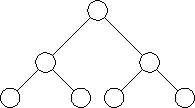
\includegraphics[width=0.3\textwidth]{figures/pamcluster.pdf}
    \hspace{1cm}
    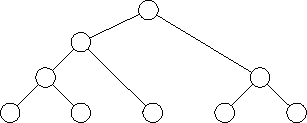
\includegraphics[width=0.3\textwidth]{figures/aggcluster.pdf}
    \caption{\label{fig:cluster_example}Example clustering results of two clustering algorithms. Left panel displays example for k-Medoids algorithm, and right panel displays example for agglomerative hierarchical clustering algorithm.}
\end{figure}


\subsection{Random hierarchies}
\label{sec:random}
 
Cluster hierarchies can potentially affect forecast performance in two aspects. First, clustering analysis creates time series that is easy to forecast, allowing original series to borrow strength. The accuracy decrease during reconciliation occurs on the newly created time series instead of the original series. Secondly, the enriched structure reduce data and model uncertainty within the base forecasts of bottom level, leading to improved reconciled forecasts.

To systematically explore these two aspects, we introduce two randomized methods for constructing hierarchies. These methods allow us to eliminate the influence of clustering and focus specifically on investigating the second aspect. 
The first approach generates hierarchies akin to those produced by k-Medoids clustering algorithms. Given $m$ bottom-level series and the number of groups $k$, it first randomly assigns $ \lfloor \frac{m}{k}\rfloor$ number of series to each group. The remaining $m -  k\times\lfloor\frac{m}{k}\rfloor$ series are then shuffled and assigned to the first $m -  k\times\lfloor\frac{m}{k}\rfloor$ groups one by one. 
This straightforward yet efficient approach constructs a three-level random hierarchy, ensuring the numbers of bottom-level series of these groups  are as nearly equal as possible, allowing us to focus solely on the impact of enriched structure on the forecast reconciliation performance. 

The second approach generates random hierarchies based on a given hierarchy, such as one constructed from clustering results. Given a hierarchy tree, it creates new hierarchies by randomly permuting the leaf nodes. In other words, it shuffles the columns of the constraint matrix $\boldsymbol{A}$ of the given hierarchy. This method yields a random ``twin'' hierarchy with the same tree structure but different groupings. If the randomized version of a cluster hierarchy significantly outperforms its original counterpart, it suggests that the second aspect holds greater importance than the first, and vice versa. Figure~\ref{fig:aggcluster_random} shows an example of this approach. The left hierarchy is the hierarchy shown in right panel of Figure~\ref{fig:cluster_example} The right hierarchy is an example of a random ``twin'' hierarchy.

\begin{figure}
    \centering
    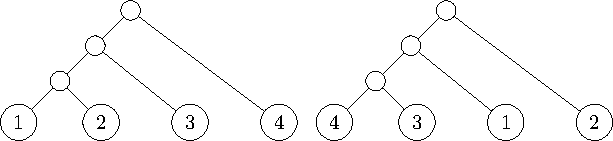
\includegraphics[width=0.8\textwidth]{figures/aggcluster_random.pdf}
    \caption{\label{fig:aggcluster_random}Examples of randomization of a given hierarchy. Right hierarchy is obtained by shuffling the leaf nodes of left hierarchy.}
\end{figure}

\subsection{Combination hierarchies}
\label{sec:combination}

To mitigate the uncertainty introduced by random hierarchies, we propose to combine multiple hierarchies. This strategy involves two primary methods. The first method focuses on combining the structures of these hierarchies. Assume there are $l$ hierarchies in the combination pool, it does so by constructing a new HTS with a summing matrix, which is a composite of the constraint matrices $\boldsymbol{A}_1, \dots, \boldsymbol{A}_l$ of  these hierarchies, along with the original constraint matrix $\boldsymbol{A}$ and the identity matrix $\boldsymbol{I}_m$. The summing matrix is thus represented as: 
\[
  \boldsymbol{S} = \begin{bmatrix}
    \boldsymbol{A} \\ \boldsymbol{A}_1 \\ \vdots \\ \boldsymbol{A}_l \\ \boldsymbol{I}_m
  \end{bmatrix}.  
\] An example of this approach is seen in the work of \cite{pangHierarchicalElectricityTime2022}, where multiple clusterings obtained from k-Means algorithms with different number of clusters are combined. 
However, this method faces challenges, particularly as the number of hierarchies in the combination pool increases, which not only raises computational time but also amplifies the uncertainty in estimating the covariance matrix.
To address this concern, \cite{pangHierarchicalElectricityTime2022} impose sparse penalty to select ideal clusters that are helpful for reconciliation.

Given the complexities of the first method, our paper concentrates on the second approach, which combines reconciled forecasts from different hierarchies. Firstly, we produce reconciled forecasts for each hierarchy. The reconciled forecasts of the original series are then extracted and combined using equal weights. Note that the resulted forecasts are still coherent. While it is possible to employ more complex methods to determine ``optimal'' weights, we adhere to equally-weighted combination due to its simplicity and well-known efficacy (\citealp{wangForecastCombinations50year2022}).

\subsection{Forecast reconciliation and evaluation}
\label{sec:reconciliation}

This subsection introduces the forecast reconciliation approach used in our paper. Assume we are making $h$-step-ahead forecasts based on $T$ historic observations for a given hierarchy $\boldsymbol{y}^c$, which could be the original hierarchy, a cluster hierarchy or a random hierarchy. 
We first produce $h$-step-ahead base forecasts $\hat{\boldsymbol{y}}^c_{T+h}$ using arbitrary forecasting models for each time series in the hierarchy. Subsequently, the minimum trace (MinT, \citealp{wickramasuriyaOptimalForecastReconciliation2019}) reconciliation method is applied to produce coherent forecasts:
\[
    \tilde{\boldsymbol{y}}_{T+h}^c = (\boldsymbol{S}'\boldsymbol{W}_h^{-1}\boldsymbol{S})^{-1}\boldsymbol{S}'\boldsymbol{W}_h^{-1}\hat{\boldsymbol{y}}_{T+h}^c,
\]
where the superscript $c$ of $\boldsymbol{S}^c$ is omitted for ease of expression. $\boldsymbol{W}_h$ is the covariance matrix of $h$-step-ahead forecast errors. We employ the shrinkage estimator of $\boldsymbol{W}_h$ proposed by \cite{wickramasuriyaOptimalForecastReconciliation2019}, which estimates the covariance matrix based on the in-sample one-step-ahead forecast errors.
Specifically, it sets  $\boldsymbol{W}_h = \lambda \hat{\boldsymbol{W}}_{1,D} + (1-\lambda)\hat{\boldsymbol{W}}_1$, where $\hat{\boldsymbol{W}}_1$ is the unbiased sample covariance estimator of the in-sample one-step-ahead forecast errors. $\hat{\boldsymbol{W}}_{1,D}$ is a diagonal matrix comprising the diagonal entries of $\hat{\boldsymbol{W}}_1$. $\lambda$ is a shrinkage intensity parameter proposed in \cite{SchaferStrimmer2005}. 

Given our specific interest in the performance of the original series, we extract reconciled forecasts of the original series from $\tilde{\boldsymbol{y}}_{T+h}^c$, i.e.,
\[
  \tilde{\boldsymbol{y}}_{T+h} = \tilde{\boldsymbol{y}}^c_{T+h, 1:(n-m) \cup (n_c - m + 1): n_c},
\]
where $n_c$ is the number of time series in the hierarchy. For combination hierarchies, the reconciled forecasts from $l$ hierarchies in the combination pool are equally combined to obtain the final forecasts, i.e.,
\[
  \tilde{\boldsymbol{y}}_{T+h}^{\text{comb}} = \frac{1}{l} \sum_{j=1}^l \tilde{\boldsymbol{y}}_{T+h}^j.
\]
Finally, these forecasts are used for evaluating the performance of different approaches.

\section{Simulation}
\label{sec:simulation}

Recall our hypothesis positing that the performance of cluster hierarchies is influenced predominantly by two aspects. The first aspect is the generation of accurate base forecasts by the newly created time series, while the second aspect is attributable to the enriched structure. In this section, we simulate two artificial scenarios using the same dataset but varying base forecasting models. The first scenario is designed to demonstrate a context where the second aspect plays a dominant role. Conversely, the second scenario is constructed to illustrate a situation where the first aspect is the predominant factor.  


\subsection{Simulation design}

\subsubsection*{Time series generation}

We assume the bottom-level time series follow an additive time series pattern with a data generating process described as follows:
\begin{equation}
    \label{simu:DGP}
    \begin{aligned}
    Y_t &= L_t + S_t + \xi_t \\
    S_t &= S_{t~\text{mod}~s} \\
    L_t &= a t + \varepsilon_t,
    \end{aligned}
\end{equation}
where $L_t$ represents the trend term which increases or decreases over time at a slope of $a$. The seasonal component, denoted by $S_t$, is repeating and deterministic with a cycle of length $s$. Both $\xi_t$ and $\varepsilon_t$ are white noises.


Instead of employing cluster algorithms, we artificially craft $6$ ideal clusters by manipulating the directions of the trend components and patterns of the seasonal components.
The configurations for each cluster can be found in Table~\ref{table:simu_params}. To simulate an increasing trend, we set the slope $a$ to $0.001$, and for a decreasing trend, we set $a$ to $-0.002$. The variances of the associate white noise $\varepsilon_t$ are set to $2.5\times 10^{-5}$ and $4.9\times 10^{-5}$ for increasing trend and decreasing trend, respectively. For series without trend (``None''), the trend component $L_t$ is set to zero. The terms ``Even'' and ``Odd'' in our setup refer to the positioning of seasonal peak. Specifically, ``Even'' seasonality means that peaks occur at even-numbered positions (e.g., $2, 4, \dots$) of seasonal cycle, with the reverse being true for ``Odd'' seasonality. The values of these seasonal peaks and troughs are randomly drawn from uniform distributions within the ranges of $[2, 3]$ and $[0,1]$, respectively. The variance of $\xi_t$ is set to $0.25$. We generate monthly time series data, ensuring that each cluster contains $20$ distinct time series. For each series, we generate $144$ observations, and the last $12$ observations are reserved for evaluation purpose. Figure~\ref{fig:simu_emps} displays example time series from each cluster, while Figure~\ref{fig:simu_pca} visualizes these generated time series based on the first two principal components extracted from principal component analysis of the series.

\begin{table}
\caption{\label{table:simu_params}Parameter setting for all clusters in the simulation experiments.}
\centering
\begin{tabular}{lcccccc}\toprule
& Cluster 1 & Cluster 2 & Cluster 3 & Cluster 4 & Cluster 5 & Cluster 6 \\
Trend & Increase & Increase & None & None & Decrease & Decrease \\
Seasonality & Odd & Even & Odd & Even & Odd & Even  \\
    \bottomrule
\end{tabular}
\end{table}

\begin{figure}
\centering
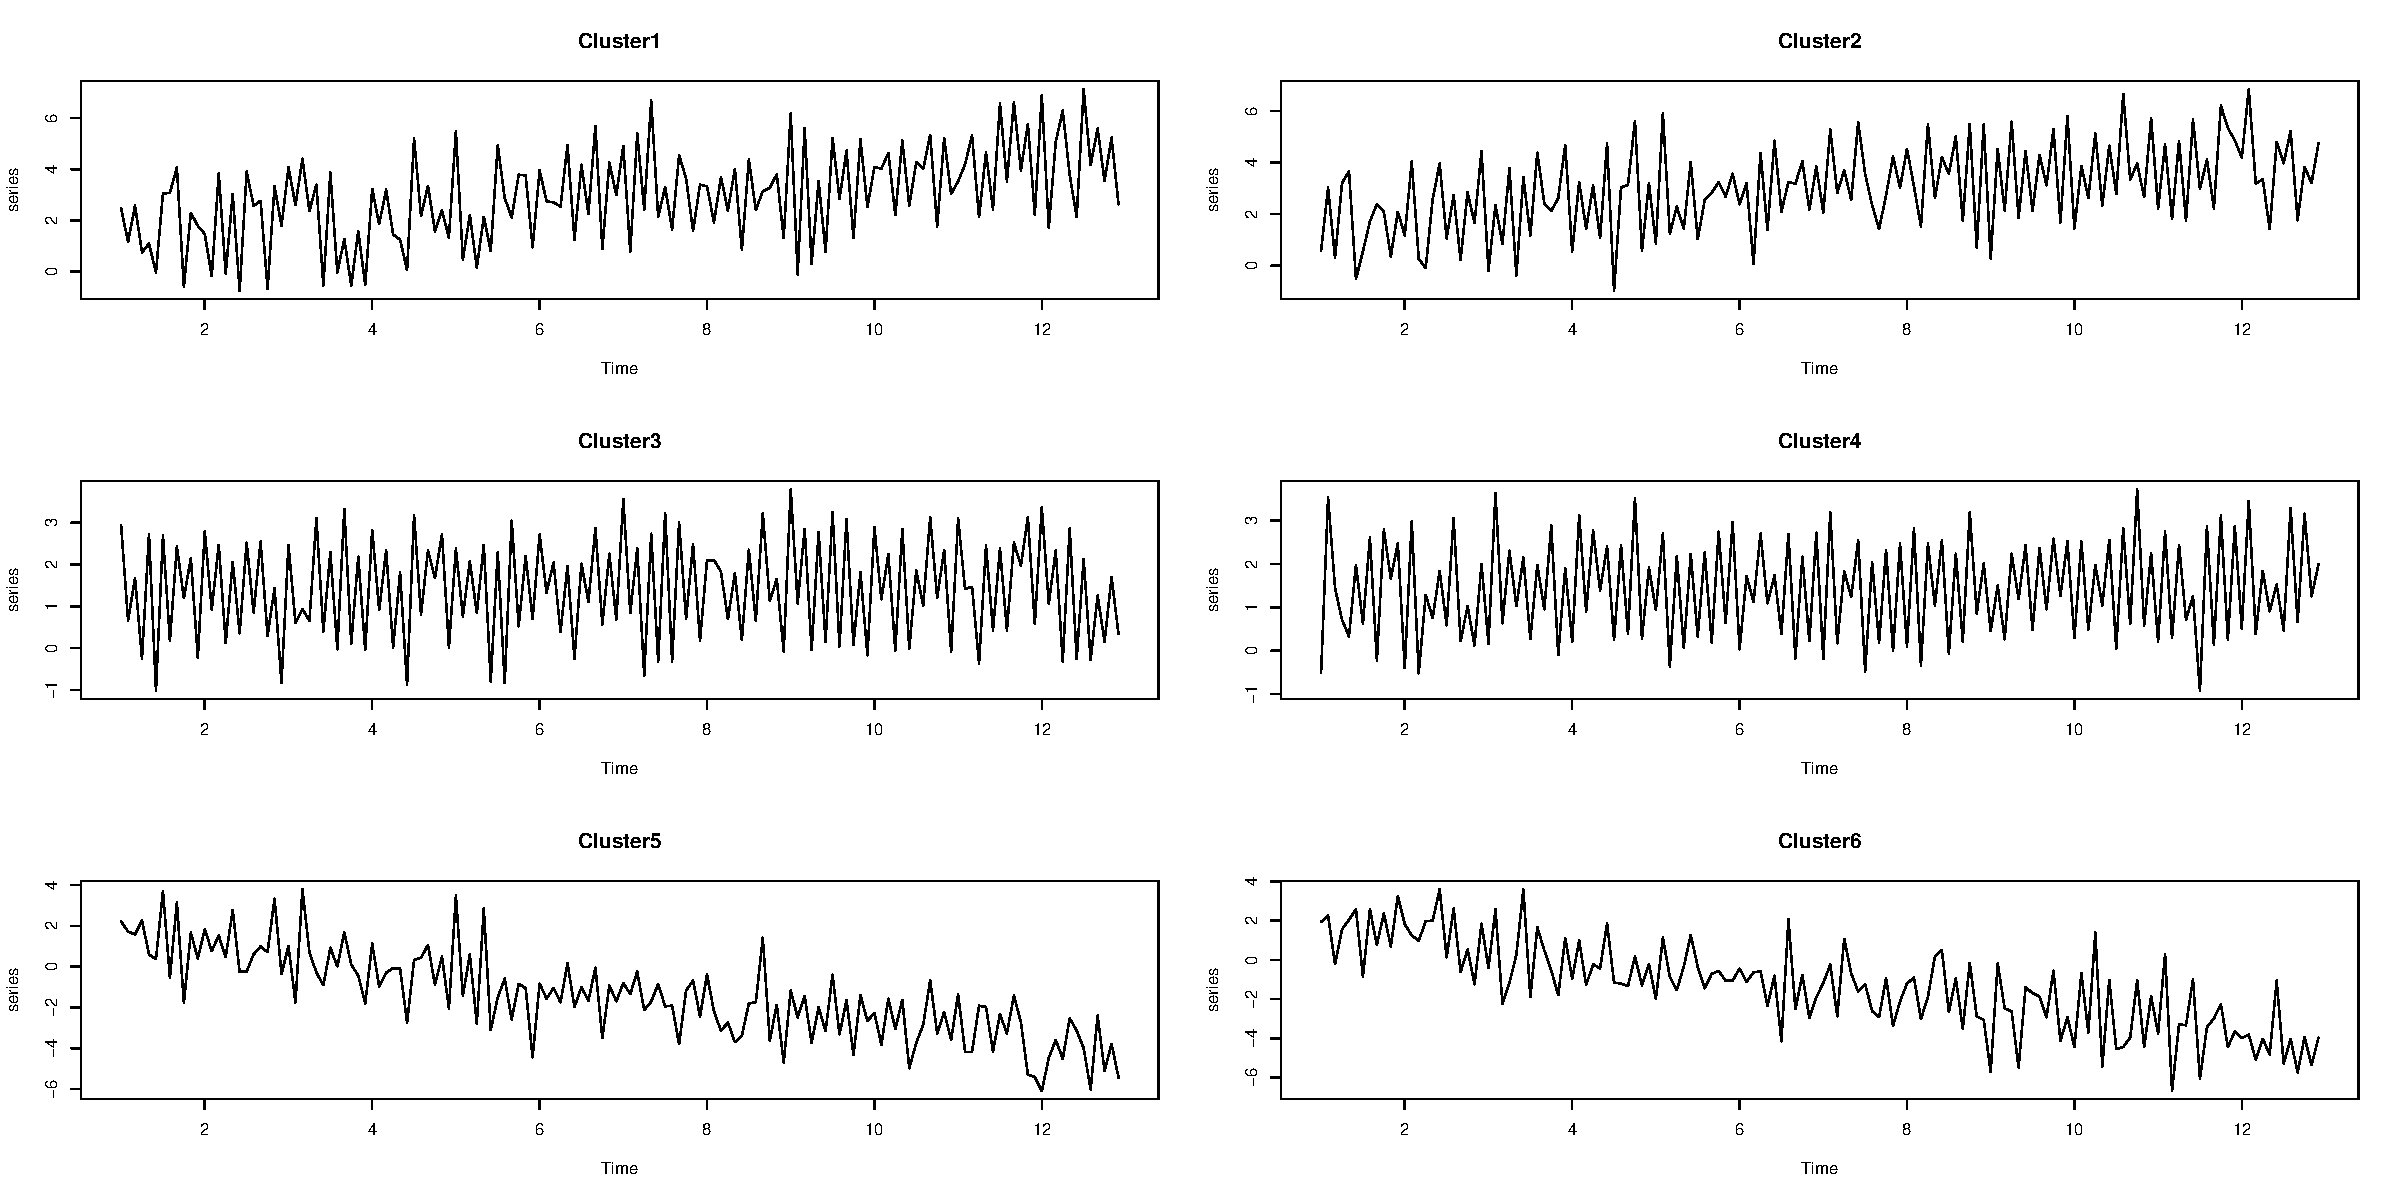
\includegraphics[width=\textwidth]{figures/simu_example.pdf}
\caption{\label{fig:simu_emps}Example time series for each cluster in the simulation experiments.}
\end{figure}

\begin{figure}
    \centering
    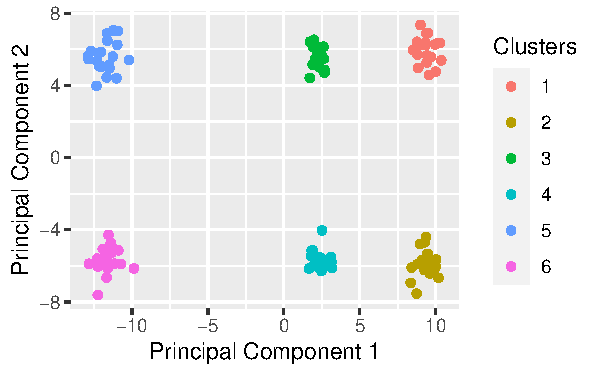
\includegraphics[width=0.6\textwidth]{figures/simu_pca.pdf}
    \caption{\label{fig:simu_pca}Visualization of the generated time series in the simulation experiments.}
\end{figure}

\subsubsection*{Hierarchies construction}

We consider an original hierarchy with a total of $120$ bottom-level series and a single aggregated series, labelled as ``C0''. In addition, we examine four cluster hierarchies and two combination hierarchies. Note that we consider multiple cluster hierarchies in order to reflect the real-world scenario where a variety of clustering techniques may be employed. The first cluster hierarchy, ``C1'', forms six middle-level series according to the predefined ideal clusters. We then merge clusters with the same trend pattern, resulting in the cluster hierarchy with three clusters, denoted by ``C2''. Similarly, we construct cluster hierarchies ``C3'' and ``C4'' based on the presence of the trend term and seasonal peak positioning, resulting in $2$ and $3$ middle-level series, respectively. Combination hierarchy ``A1'' combines reconciled forecasts obtained from all four cluster hierarchies (``C1'' to ``C4'') using equal weights. Moreover, by shuffling the bottom-level series within the cluster hierarchy ``C1'', we generate random ``twin'' hierarchies, as described in Section~\ref{sec:random}. The second combination hierarchy ``A2'' combines reconciled forecasts from ten random ``twin'' hierarchies using equal weights.

\subsubsection*{Forecasting}

Given the generated hierarchies, we construct two distinct scenarios, each employing different base forecasting models. In the first scenario, exponential smoothing (ETS, \citealp{ForecastingExponentialSmoothing}) is used to generate base forecasts for all time series in hierarchies. This setup simulates a context where raw time series are used as time series representations for clustering.
In the second scenario, we apply the historic mean for generating base forecasts for the bottom-level series, while continuing to use ETS for other time series in hierarchies. This approach ensures that the in-sample forecast errors exhibit patterns similar to those of the raw time series, simulating the scenario where in-sample forecast errors are considered as time series representations for clustering. Furthermore, this scenario aims to verify the proposition that the original series can borrow strength from the newly created series. We refer to these scenarios as ``clustering by time series'' and ``clustering by error'', respectively. 


\subsection{Evaluation}
\label{sec:simu_eval}

Recalling that our purpose is to improve forecast performance of the original series, our evaluation focuses exclusively on reconciled forecasts of the total-level and bottom-level series. 
Firstly, we employ the Root Mean Squared Error (RMSE) as our accuracy metric for forecasts of individual time series. 
To ensure robustness and reliability in our findings, we conduct the simulation $500$ times, resulting in a comprehensive evaluation set comprising $500\times 121$ RMSEs for each hierarchy. 
Multiple comparisons with the best (MCB) test is then applied to compute the average ranks of the seven hierarchies as well as the base forecasts, and to determine whether the performance differences are statistically different (\citealp{tsutils}).


\subsection{Results}
\label{sec:simu_res}

Figure~\ref{fig:simu_mcb} presents the MCB test results for both scenarios. The results reveal that in both scenarios, most approaches perform better than the base forecasts and the original two-level hierarchy ``C0''. This outcome indicates that hierarchy construction generally improves forecast reconciliation performance, corroborating similar findings reported in existing literature, such as those by \cite{pangHierarchicalElectricityTime2022,liForecastReconciliationApproach2019} and \cite{matteraImprovingOutofSampleForecasts2023}.


In the ``clustering by time series'' scenario, the ideal cluster ``C1'' achieves a $4$th rank, indicating that optimal clustering does not necessarily translate into the best forecast reconciliation performance. 
On the other hand, ``C1'' ranks $1$st in the ``clustering by error'' scenarios and demonstrates superior performance over other clustering approaches and its randomized counterpart. This finding implies that in this scenario, the created series based on clustering, as opposed to enriched structure, plays a crucial role in improving forecast performance.
However, it is important to recognize that such scenarios may be uncommon in practical applications due to careful modeling of base forecasts. Thus, the in-sample forecast errors in practice may not exhibit clear patterns as those observed in this simulation, leading to clustering with more uncertainty.
Additionally, the varying  performance of ``C1'' across two scenarios highlight the significance of carefully selecting time series representations when constructing new middle levels using clustering algorithms.


Regard the combination hierarchies, it is noteworthy that the equally weighted combination of ten random hierarchies achieves first rank in the first scenario. Meanwhile, the equally weighted combination of four clustering hierarchies ranks third in both scenarios. These outcomes suggest that forecast combination can further improve forecast performance of both random hierarchies and cluster hierarchies. Interestingly, in the first scenario, the combination of random hierarchies outperforms the combination of cluster hierarchies in. This implies that the enriched structure has a more significant impact on forecast performance in this context. We argue that this outcome can be attributed to the already high quality of base forecasts, as indicated by the close relative ranks of the various approaches.  When the base forecasts are sufficiently accurate, the added value of reconciliation through complex hierarchical structures might be limited, while combination of hierarchies further improves performance by dealing with data and model uncertainty.

In summary, our simulation effectively illustrates two distinct scenarios, each highlighting a separate factor contributing to the performance improvement offered by hierarchy contribution approaches. However, it is crucial to acknowledge that both scenarios represent simplified, somewhat exaggerated representations of practical situations. The actual practice of forecasting involves careful modeling, but is also impacted by ubiquitous model misspecification, which adds complexity that isn't fully captured in these artificial scenarios. To further validate and explore the effectiveness of various methodologies, we will conduct experiments on two real-world applications, thereby offering a more practical and nuanced understanding of these approaches.


\begin{figure}
    \centering
    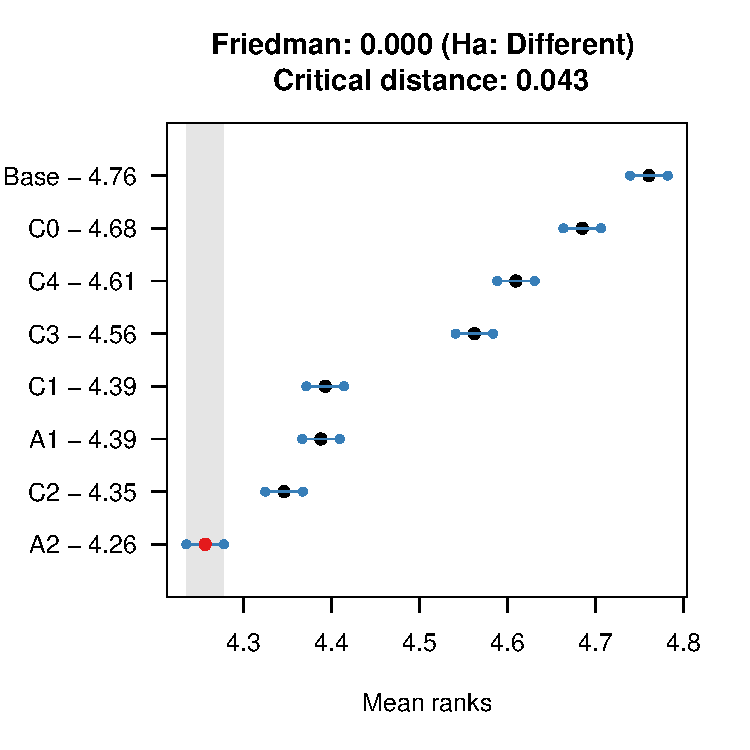
\includegraphics[width=0.45\textwidth]{figures/simu_mcb1.pdf}
    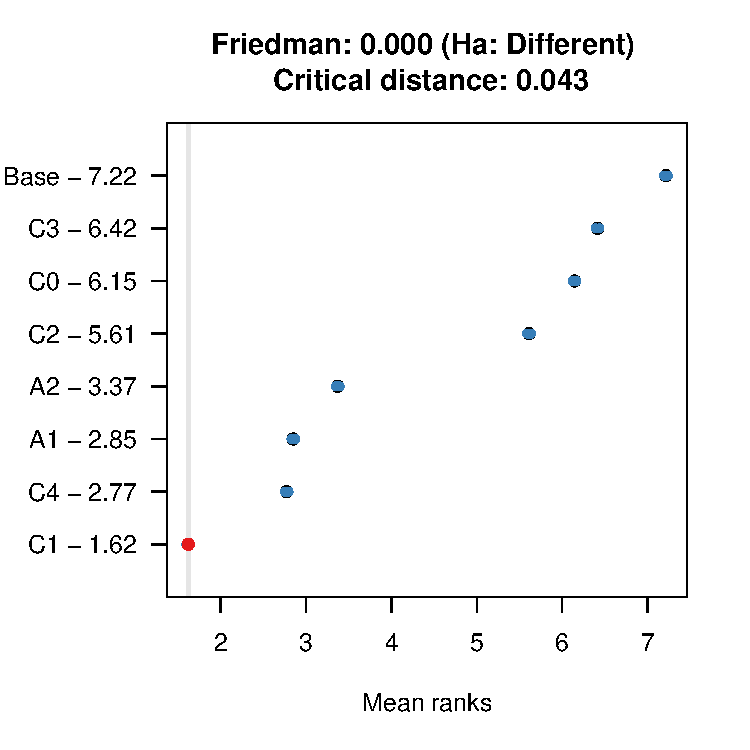
\includegraphics[width=0.45\textwidth]{figures/simu_mcb2.pdf}
    \caption{\label{fig:simu_mcb}Average ranks and 95\% confidence intervals based on the MCB Test for the $8$ approaches in the two scenarios of the simulation experiments. Left panel displays test results for the ``clustering by time series'' scenario and right panel displays test results for the ``clustering by error'' scenario.}
\end{figure}

\section{Empirical studies}
\label{sec:emp}
\subsection{Datasets}

We analyze two datasets in our empirical studies. The first dataset is the monthly Australian domestic tourism dataset, covering the period from January 1998 to December 2016. The tourism demand of Australia is geographically disaggregated into seven states and territories, which are further divided into $27$ zones and $76$ regions. Additionally, each geographical series is divided by four travel purposes (\citealp{wickramasuriyaOptimalForecastReconciliation2019}). Overall, this dataset comprises a total of $555$ time series with $304$ of those at the bottom level.

The second dataset focuses on causes of death in the United States, using the ICD 10 coding system. We obtain monthly cause-specific death count data from the Center for Disease Control and Prevention (CDC) for the period between 1999 and 2019. The coding system inherently forms an unbalanced hierarchy containing $137$ time series, with $113$ of those being bottom-level series. To address issues with suppressed data values, we combine causes that contain missing values and share a parent cause. The death counts for these combined categories are calculated by subtracting the death counts of sibling causes from the death counts of their parent cause. This processing results in a refined dataset that includes $120$ time series with $98$ at the bottom level.

\subsection{Experiment design}

In our analysis of the two datasets, we focus specifically on the total-level and bottom-level series rather than evaluating all levels of the given hierarchies. These two-level hierarchies are referred to as ``original hierarchy'', serving as our benchmark. The given hierarchy, referred to as ``natural hierarchy'', is considered as one way of hierarchy construction that is based on metadata of the time series. We demonstrate that for the purpose of forecast performance, the natural hierarchy may not be the most effective hierarchical structure.

Regarding cluster hierarchies, we employ twelve time series techniques which are derived from combinations of four time series representations, two distance measures and two clustering algorithms. The names and details of these approaches are listed in Table~\ref{tab:emp_method}. The four time series representations need to perform dimension reduction when using Euclidean distance, as we have discussed in Section~\ref{sec:clustering}. Combing the four dimension reduced representations with two clustering algorithms results in the first eight clustering approaches. Features of raw time series and in-sample forecast error are not temporal data, thus incompatible with DTW. The last four approaches are derived from combinations of two temporal representations, two clustering algorithms and DTW.


\begin{table}
\caption{\label{tab:emp_method} Hierarchy construction approaches used in empirical studies.}
\centering
\resizebox{\textwidth}{!}{
\begin{tabular}{ccccc}
    \toprule
    Approaches & Representation & Dimension reduction & Distance measure & Clustering algorithms  \\
    TS-MED & Raw time series & Yes & Euclidean & k-Medoids \\
    ER-MED & In-sample error & Yes & Euclidean & k-Medoids \\
    TSF-ME & Raw time series features & Yes & Euclidean & k-Medoids \\
    ERF-ME & In-sample error features & Yes & Euclidean & k-Medoids \\
    TS-HC & Raw time series & Yes & Euclidean & hierarchical clustering  \\ 
    ER-HC & In-sample error & Yes & Euclidean & hierarchical clustering  \\ 
    TSF-HC & Raw time series features & Yes & Euclidean & hierarchical clustering  \\ 
    ERF-HC & In-sample error features & Yes & Euclidean & hierarchical clustering  \\
    TS-MED-DTW & Time series & No & DTW & k-Medoids \\
    TS-HC-DTW & In-sample error & No & DTW & hierarchical clustering \\
    ER-MED-DTW & Time series & No & DTW & k-Medoids \\
    ER-HC-DTW & In-sample error & No & DTW & hierarchical clustering 
     \\\bottomrule
\end{tabular}}
\end{table}

Additionally, we explore three combination hierarchies. The first one, referred to as ``FC-R'', implements the first random hierarchy construction approach outlined in Section~\ref{sec:random}. Here, we set the number of groups $k$ to $15$, an arbitrary number chosen with the goal of creating a moderate number of groups, each containing a moderate number of series.
We repeat this process to create ten similar hierarchies and combine their reconciled forecasts using equal weights.
This approach is employed to verify the hypothesis that hierarchy construction can improve forecast reconciliation performance.
The second combination hierarchy, denoted by ``FC-N'', adopts the alternative random hierarchy construction approach also discussed in Section~\ref{sec:random}. Specifically, we randomly create ten ``twin'' hierarchies of the natural hierarchy, to evaluate our argument that the natural hierarchy might not be the optimal hierarchy in terms of forecast performance.
The third combination hierarchy, labelled by ``FC-C'', involves an equally-weighted combination of the reconciled forecasts obtained from the $12$ cluster hierarchies shown in Table~\ref{tab:emp_method}. This approach aims to demonstrate that the performance of hierarchy construction approaches can be further enhanced through forecast combination.

The time series features used in this experiment are calculated using the \texttt{tsfeatures} package (\citealp{tsfeatures}) for R (\citealp{R}). After filtering out the features that are constant across all series, $56$ features are reserved. The k-Medoids and hierarchical clustering algorithms are implemented using the \texttt{cluster} (\citealp{cluster}) package for R. The base forecasts are generated using the automatic ETS models, which are then reconciled using the minimum trace method with shrinkage estimator.

To rigorously validate our hypothesis, we utilize the rolling window strategy to evaluate the performance of different approaches on both datasets. We begin by fitting base forecasting models using the first $96$ observations. Then we calculate time series representations and construct new hierarchies, either through clustering or random approaches, and then forecast $12$ steps ahead. After that, the training set is increased by one observation and new forecasts are obtained. The procedure is repeated until the last $12$ observations are used for evaluation. Finally, we can obtain $121$ $12$-step-ahead forecasts for the tourism dataset and $144$ $12$-step-ahead forecasts for the mortality dataset. 

We compare the forecast performance of the twelve cluster hierarchies, three combination hierarchies as well as the natural hierarchy, the original two-level hierarchy and base forecasts. Same as the evaluation measure described in Section~\ref{sec:simu_eval}, we first calculate RMSE for each of the $12$-step-ahead forecasts, resulting in $144 \times 99$ RMSE values for the mortality dataset and $121 \times 305$ RMSE values for the tourism dataset for each approach. We then conduct the MCB test on these RMSE values to statistically assess the differences in forecast accuracy.

\subsection{Results}

The MCB test results for the tourism dataset and mortality dataset are shown in Figure~\ref{fig:tourism_mcb} and Figure~\ref{fig:mortality_mcb}, respectively. For both datasets, most hierarchy construction approaches outperform both base forecasts and the two-level hierarchy. The first combination approach ``FC-R'' achieves third rank on the mortality dataset eighth rank on the tourism dataset. These results demonstrate that hierarchy construction can enhance forecast performance, further supporting the findings in our simulation and the literature. 

In both datasets, the evidence suggests that the natural hierarchy may not be optimal for performance. The equally weighted combination of "twin" hierarchies derived from the natural hierarchy (``FC-N'') outperform the natural hierarchy itself, supporting this hypothesis.  This finding reinforces our belief that better hierarchical structures can be constructed, as evidenced by the superior performance of some cluster hierarchies on the tourism dataset. 
Most cluster hierarchies outperform the original two-level hierarchy on both datasets, further demonstrating the effectiveness of clustering approaches. However, three exceptions on the mortality dataset highlight the importance of choosing an appropriate clustering technique.

Interestingly, unlike the simulation where either clustering or enriched structure play the primary role in performance improvement, both factors contribute to better forecasts in the two real-world datasets.  First, the randomized natural hierarchy ``FC-N'' outperform all  cluster hierarchies and the natural hierarchy on both datasets, showcasing the benefit of enriched structure. Second, the equally weighted combination of cluster hierarchies achieves the top rank, demonstrating the effectiveness of clustering techniques. 
Furthermore, the impressive performance of the three combination hierarchies underscores the potential of combining forecasts from multiple hierarchies for even greater accuracy. This suggests that the impact of combination may even more significant than the individual contributions of clustering and enriched structure.

\begin{figure}
    \centering
    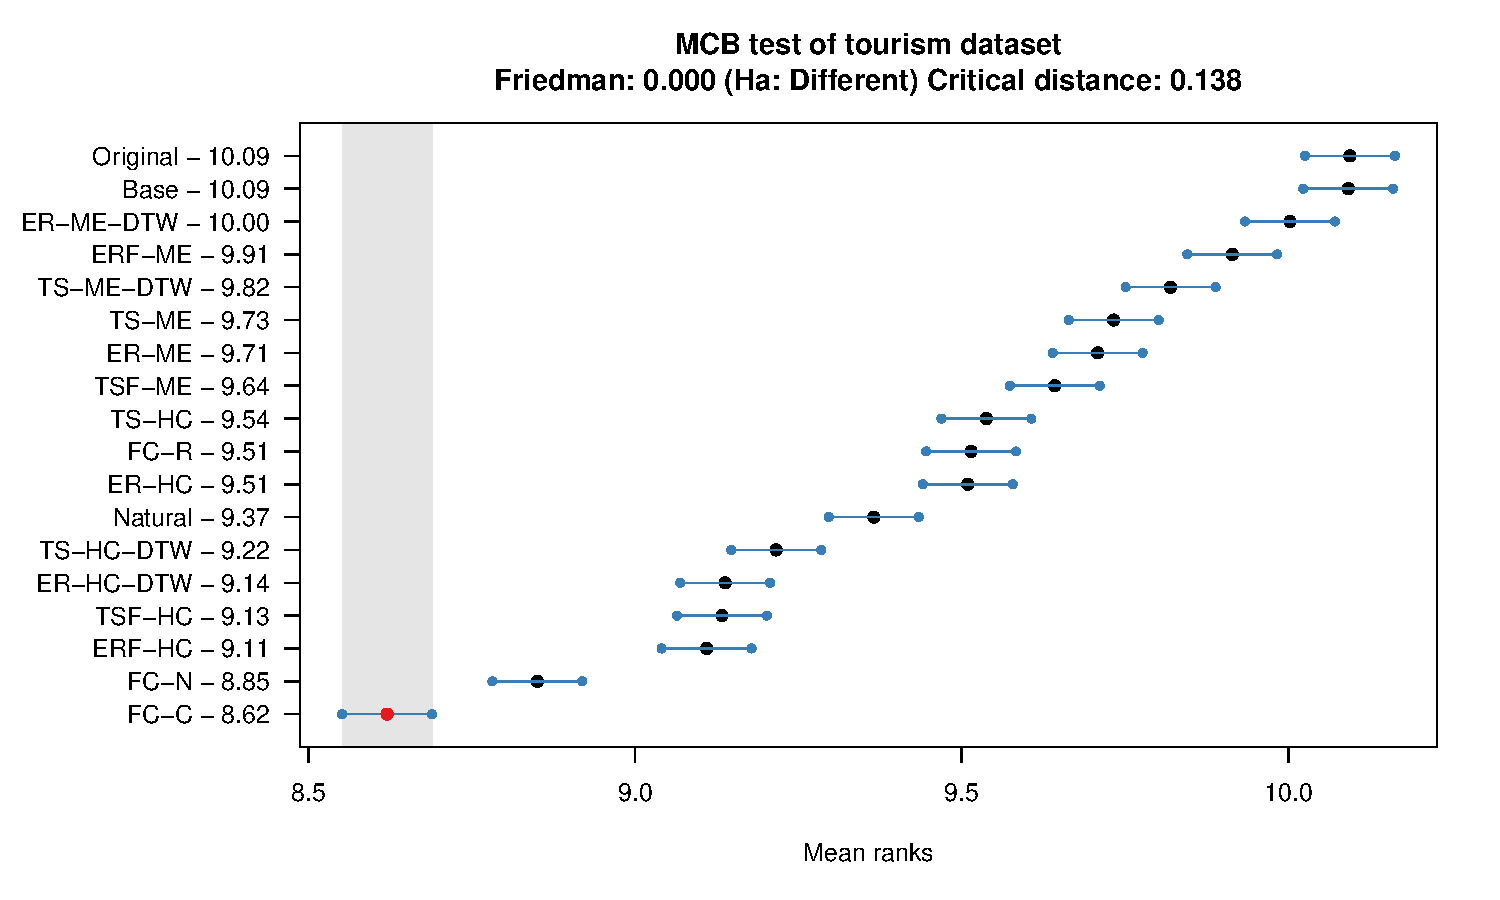
\includegraphics[width=\textwidth]{figures/tourism_mcb.pdf}
    \caption{\label{fig:tourism_mcb}Average ranks and 95\% confidence intervals based on the MCB Test for the $18$ approaches on the tourism dataset.}
\end{figure}

\begin{figure}
    \centering
    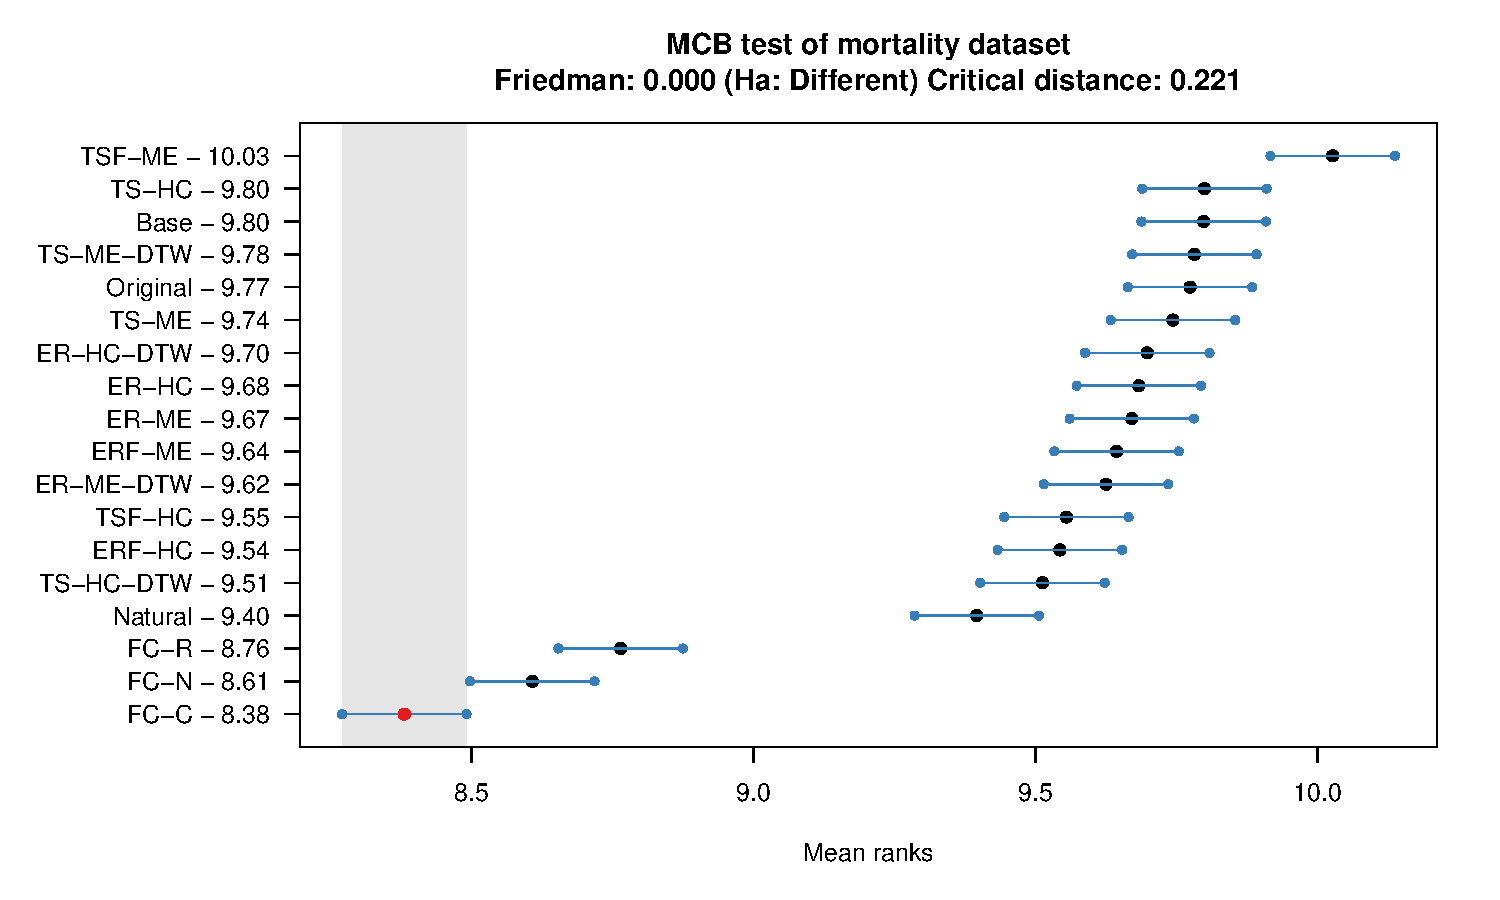
\includegraphics[width=\textwidth]{figures/mortality_mcb.pdf}
    \caption{\label{fig:mortality_mcb}Average ranks and 95\% confidence intervals based on the MCB Test for the $18$ approaches on the mortality dataset.}
\end{figure}

The approach based on hierarchical clustering outperforms the approach based on k-Medoids on the tourism dataset when using the same representation and distance metric, e.g., ``TSF-HC'' significantly outperforms ``TSF-ME''. However, this is not consistently observed for every combination of representation and distance metric on the mortality dataset. We believe this discrepancy is due to different time series patterns at the bottom level of these two datasets.
In the case of the mortality dataset, we combine rare causes of death that have suppressed values and record death counts at a national level. As a result, most series at the bottom level exhibit strong seasonality and trend. On the other hand, in the tourism dataset, the tourism demand is disaggregated for both travel purposes and geographical regions. This leads to numerous bottom-level series with high volatility and many zeros, making them more challenging to forecast.
Therefore, having a hierarchy with more middle-level series can be more advantageous for reconciliation in the tourism dataset compared to the mortality dataset. Additionally, we suspect that the inferior performance of ``FC-R'' on the tourism dataset may be partly attributed to an insufficient number of middle-level series.

In most cases, the in-sample error representation outperforms the time series representation when using the same distance metric and clustering algorithms. However, this performance difference is not as significant as what was observed in Section~\ref{sec:simu_res}. Intuitively, hierarchies constructed based on clustering in-sample error should be similar to random hierarchies when all base models are correctly specified. However, due to ubiquitous model misspecification in practice, vague patterns emerge in the in-sample error, which leads to contradictory results.


\subsubsection*{Effect of number of random hierarchies}

In our previous experiments, we set the number of random hierarchies in ``FC-R'' and ``FC-N'' to $10$ for fair comparisons with ``FC-C''. However, we believe that increasing the number of random hierarchies could further enhance performance. In this subsection, we explore the effects of using 20 and 50 random hierarchies, referred to as ``FC-N-20'', ``FC-N-50'', ``FC-R-20'', and ``FC-R-50''. We compare these variations with ``FC-R'', ``FC-C'', and ``FC-N'' using the same evaluation procedure described earlier. The results from the MCB test are presented in Figure~\ref{fig:number_mcb}, where the left panel shows results on the tourism dataset and the right panel displays results on the mortality dataset.

Generally, we observe that forecast performance improves as the number of random hierarchies increases, except for ``FC-N-20'' and ``FC-N'' on the mortality dataset. Surprisingly, on the tourism dataset, ``FC-N-50'' performs slightly better than ``FC-C''. It is important to note that employing more random hierarchies comes at a cost of increased computational resources. Therefore, one must carefully consider trade-offs between efficiency and performance when making decisions.

\begin{figure}
\centering
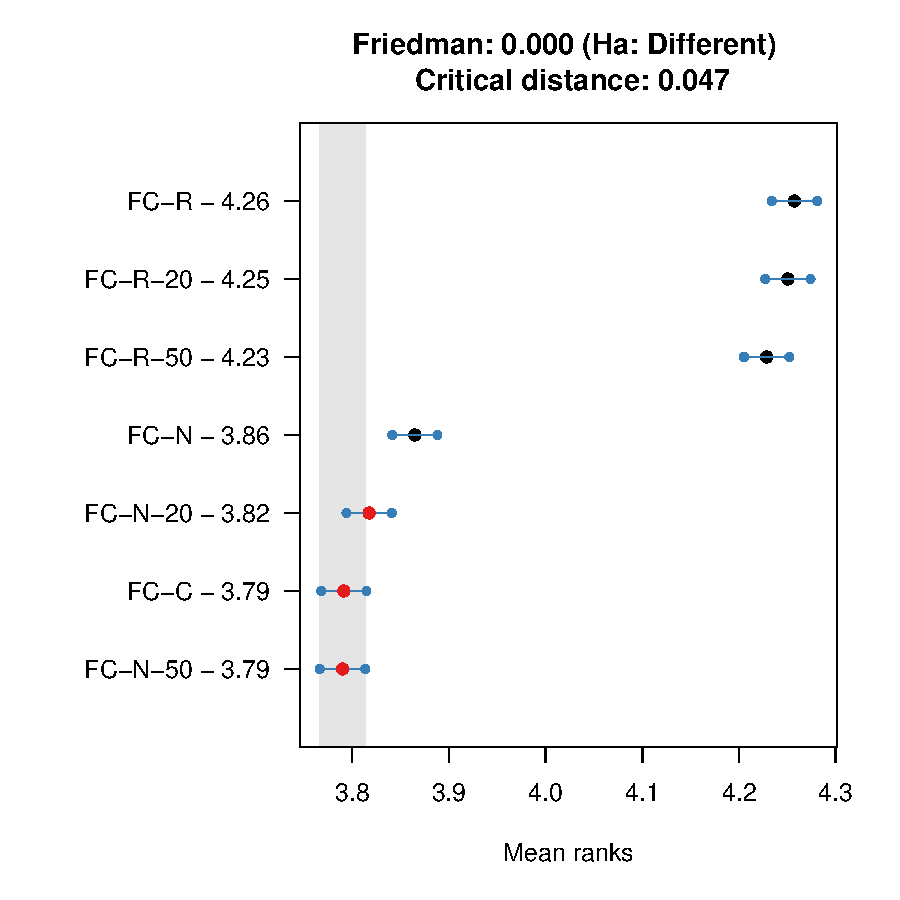
\includegraphics[width=0.45\textwidth]{figures/tourism_number_mcb.pdf}
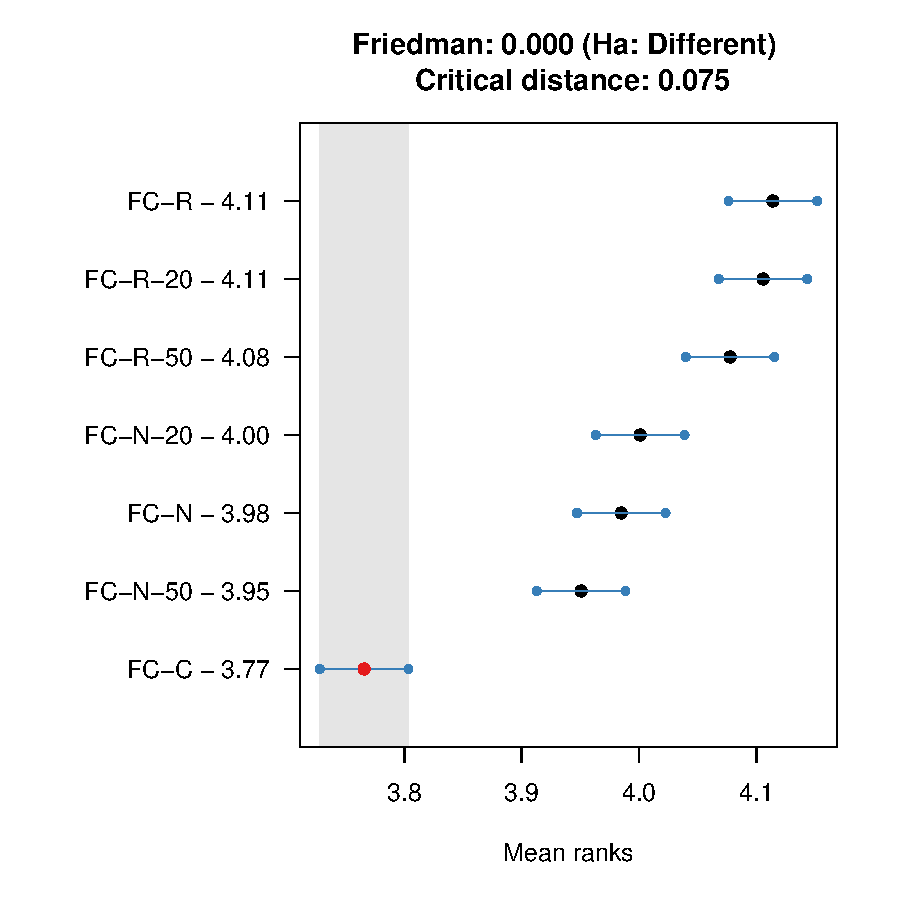
\includegraphics[width=0.45\textwidth]{figures/mortality_number_mcb.pdf}
\caption{\label{fig:number_mcb}Average ranks and 95\% confidence intervals based on the MCB Test of different number of random hierarchies on two datasets. Left and right panels display test results on tourism dataset and mortality dataset, respectively.}
\end{figure}

\section{Discussion and Conclusion}
\label{sec:conclusion}

This paper extends the current body of research on clustering-based forecast reconciliation by introducing a general hierarchical forecasting framework, incorporating three distinct approaches: cluster hierarchies, random hierarchies, and combination hierarchies.
In contrast to the focused scope of previous studies, our approach to cluster hierarchies involves a broader exploration. We examine four time series representations, employ two distance measures, and utilize two clustering algorithms. This comprehensive method differs significantly from the existing literature, which typically concentrates on specific clustering implementations.
We also introduce two innovative random hierarchy construction methods to investigate what drives the performance enhancements in cluster hierarchies. These random hierarchies help isolate the effect of clustering, allowing us to focus on the benefits derived from the enriched structure alone.
Furthermore, we propose combination hierarchies to mitigate uncertainties inherent in random hierarchies.

Our simulation study is constructed around two scenarios, each based on different base forecasting models. The first scenario highlights the value of the enriched structure, evident in the high-ranking performance of random combination hierarchies. Enriched structure can further improve forecast performance when the base forecasts are of high quality. The second scenario demonstrates the efficacy of clustering-based approaches, particularly when the base forecasts at the bottom level are less accurate.

Empirical studies on two datasets support our simulation findings. In the tourism dataset, the inferior base forecasts at the bottom level lead to all cluster hierarchies surpassing the original hierarchy, with four outperforming the combination of random hierarchies, which is used to demonstrate the impact of enriched structure. In contrast, the superior performance of two random combination hierarchies in the mortality dataset highlights the effectiveness of enriched structure. These results imply that the dominant factor, whether it is the enriched structure or clustering, varies depending on the dataset's characteristics, the base forecasting models, and other variables. Overall, our findings suggest that hierarchy construction approaches generally enhance performance, and combining these approaches leads to further improvements.


Future research based on our study could proceed in several promising directions. Firstly, our experiments were concentrated on total-level and bottom-level series. In practical applications, it might be necessary to include specific middle levels or evaluate the entire hierarchy. This could lead to the exploration of different hierarchy approaches, such as clustering middle-level series rather than bottom-level ones. Although we used equally-weighted combinations in this study, there's potential for applying more sophisticated methods to improve performance. The extensive literature on forecast combination, including advanced methods for calculating weights, offers numerous possibilities for enhancement (refer to \citealp{wangForecastCombinations50year2022} for an in-depth review).

In Section~\ref{sec:combination}, we discuss the implications of combining multiple hierarchical structures on the uncertainty in estimating the covariance matrix of base forecast errors. Our conclusion was to opt for forecast combination rather than combining the structures of the hierarchies.  However, a systematic exploration of these two strategies, combining hierarchical structures and combining forecasts, presents an intriguing area for future research. Specifically, addressing the challenge of uncertainty due to high dimensionality in the combination of hierarchical structures is possible. In this context, innovative solutions like the regularized forecast reconciliation approach, as proposed by \cite{bentaiebRegularizedRegressionHierarchical2019a}, and alternative estimators of the covariance matrix, such as those suggested by \cite{pritulargaStochasticCoherencyForecast2021} could be highly beneficial. 

In both our simulation and empirical studies, the combination of random hierarchies displayed competitive results compared to clustering-based methods. However, the efficacy of this approach in scenarios with an extremely large number of bottom-level series remains uncertain. In such cases, a partially random approach might be more effective. For instance, initially generating random hierarchies, identifying those with superior performance, and then constructing partially random hierarchies based on these well-performing structures could be a viable strategy. Another intriguing possibility is the integration of both clustering and random approaches. Moreover, our study focused specifically on the aggregation of bottom-level series, which may have constrained the potential of middle-level series. It's plausible to enhance forecastability at the middle level by creating series through general linear combinations. 


Finally, our study was centered around point forecast reconciliation and cross-sectional hierarchy. However, the field of probabilistic forecast reconciliation has recently gained significant interest, as evidenced by research like \cite{panagiotelisProbabilisticForecastReconciliation2023} and \cite{jeonProbabilisticForecastReconciliation2019}. Applying hierarchy construction approaches to probabilistic forecast reconciliation presents a novel and potentially fruitful research avenue. This approach could provide deeper insights and more robust forecast reconciliation methods, particularly in scenarios where uncertainty and variability are significant factors.
Another promising direction for extending our methodologies lies in exploring temporal (\citealp{athanasopoulosForecastingTemporalHierarchies2017}) and cross-temporal hierarchies (\citealp{girolimettoCrosstemporalProbabilisticForecast2023a}). 



\section*{Acknowledgements}

Bohan Zhang is supported by the international joint doctoral education fund of Beihang University.

\begingroup
\setstretch{1.15}
\bibliographystyle{agsm}
\bibliography{references.bib}
\endgroup



\end{document}